%\label{introductorybookmark}
%\pagebookmark[level=0]{introductorybookmark}{Vous avez dit numérique ?}
%\chapter*{Vous avez dit numérique ?}
%\addcontentsline{tdm}{chapter}{Vous avez dit numérique ?}
%\pagestyle{plain}
\backchapter{Vous avez dit numérique ?}% Avoiding a `\frontchapter' definition

\lettrine{Q}{uid du numérique ?} Le « numérique » recouvre les champs disciplinaires de l'informatique qui, de fait, est à double entrée, à voir à la fois comme une science et une technologie. 

Comme corollaires respectifs, l'informatique est également une cul\-ture et une industrie (voir une discussion détaillée sur le \href{https://pixees.fr/sur-la-definition-du-mot-numerique/}{terme numérique}), avec des usages et des conventions. 
Du reste, on distinguera les sciences \emph{du} numérique --- à savoir, informatique et mathématiques appliquées --- des sciences numériques --- autrement dit, les sciences transformées par le numérique. 

\sidegraphic[Facettes du numérique.]{%
% From: https://tex.stackexchange.com/questions/66490/drawing-a-tikz-arc-specifying-the-center
\begin{tikzpicture}
\tikzset{
  pics/carc/.style args={#1:#2:#3}{
    code={
      \draw[pic actions] (#1:#3) arc(#1:#2:#3);
    }
  }
}
%\draw[step=0.25cm,style=help lines, line width=0.1pt] (-2.5,-2.0) grid (2.5,2.0);
%\draw[step=1cm,style=help lines, line width=0.8pt] (-2.5,-2.0) grid (2.5,2.0);
%\draw[thick, dashed] (2,0) arc (-20:200:2cm);
\draw (0,0) pic[very thick, dashed, secondcolor]{carc=-20:200:2cm};
\begin{scope}[xshift=-2.0cm, scale=0.75]
	\draw[draw=firstcolor, fill=firstcolor] (-0.5,-0.25) -- (-0.5,0.25) -- (-0.25,0.5) -- (0.25,0.5) -- (0.5,0.25) -- (0.5,-0.25) -- (0.25,-0.5) -- (-0.25,-0.5) -- cycle;
\end{scope}
\begin{scope}[xshift=2.0cm, scale=0.75]
	\draw[draw=firstcolor, fill=firstcolor] (-0.5,-0.25) -- (-0.5,0.25) -- (-0.25,0.5) -- (0.25,0.5) -- (0.5,0.25) -- (0.5,-0.25) -- (0.25,-0.5) -- (-0.25,-0.5) -- cycle;
\end{scope}
\begin{scope}[yshift=2.0cm, scale=0.75]
	\draw[draw=firstcolor, fill=firstcolor] (-0.5,-0.25) -- (-0.5,0.25) -- (-0.25,0.5) -- (0.25,0.5) -- (0.5,0.25) -- (0.5,-0.25) -- (0.25,-0.5) -- (-0.25,-0.5) -- cycle;
\end{scope}
\node[anchor=west, font=\footnotesize, inner sep=0pt] at (-2.5,-1.0) {Technologie};
\node[anchor=east, font=\footnotesize, inner sep=0pt] at (2.5,-1.0) {Usages};
\node[anchor=south, font=\footnotesize, inner sep=0pt] at (0.0,2.75) {Science};
\node[anchor=center, font=\footnotesize, inner sep=0pt] at (0.0,0.0) {Culture};
\end{tikzpicture}
}{Canope}
Au-delà de la dénomination « SNT », \textit{Sciences [du] Numérique[s] et Technologie}, il faut bien comprendre que ce sont ces quatre facettes qui sont à faire découvrir aux élèves, pour leur permettre de se construire une vraie vision sur ces sujets.

L’enseignement de sciences numériques et technologie en classe de seconde a pour objet d’appréhender les principaux concepts des sciences [du] numérique[s], mais également de permettre aux élèves, à partir d’un objet technologique, de comprendre le poids croissant du numérique et les enjeux qui en découlent.

\vspace{1.2\baselineskip}
\subsubsection*{Vivre à l'ère du numérique}

La numérisation généralisée des données, les nouvelles modalités de traitement ou de stockage et le développement récent d’algorithmes permettant de traiter de très grands volumes de données numériques constituent une réelle rupture dans la diffusion des technologies de l’information et de la communication. Cette révolution multiplie les impacts majeurs sur les pratiques humaines.

\sidegraphic{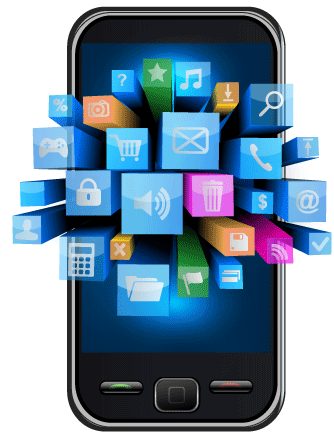
\includegraphics[width=0.75\linewidth]{./Images/Chapter00/smartphone-pngtree.png}}{pngtree.com}
Par exemple, l’actuel mobile multifonction est un objet technologique qui permet, comme le téléphone du XX\frup{e} siècle, de téléphoner, mais [qui est aussi] devenu une interface universelle d’accès à l’information et de commande d’autres objets.

La convergence d’activités utilisant le numérique est un phénomène généralisé lié au développement de la science informatique et des technologies associées et notamment à leur intégration avec le domaine des télécommunications, à l’informatisation massive de champs économiques variés (communication, audiovisuel, transports, instrumentation scientifique médicale et technique, outillage numérique, objets connectés, etc.) et, bien sûr, à la création du réseau Internet.

%\vfill\pagebreak


\subsubsection*{Concepts définis par la science informatique}

\sidegraphic[Concepts de l'informatique.]{%
\footnotesize
\textsc{Algorithme}\\[4pt]
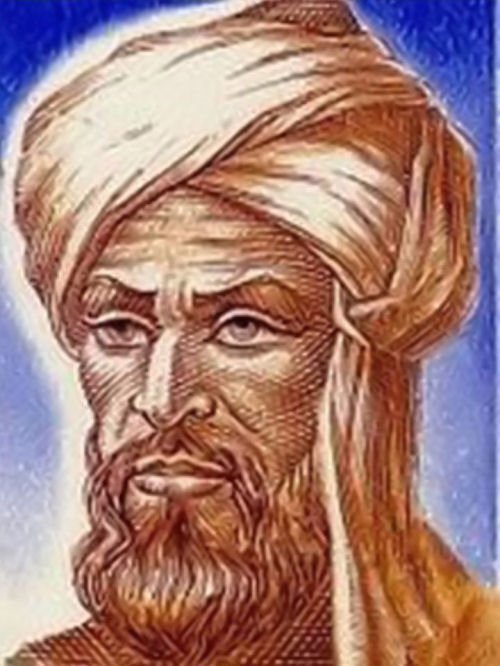
\includegraphics[width=0.725\linewidth]{./Images/Chapter00/al-khwarizmi.png}\\ Muhammad al \textsc{Khwārizmī} \\[10pt]
\textsc{Données}\\[4pt]
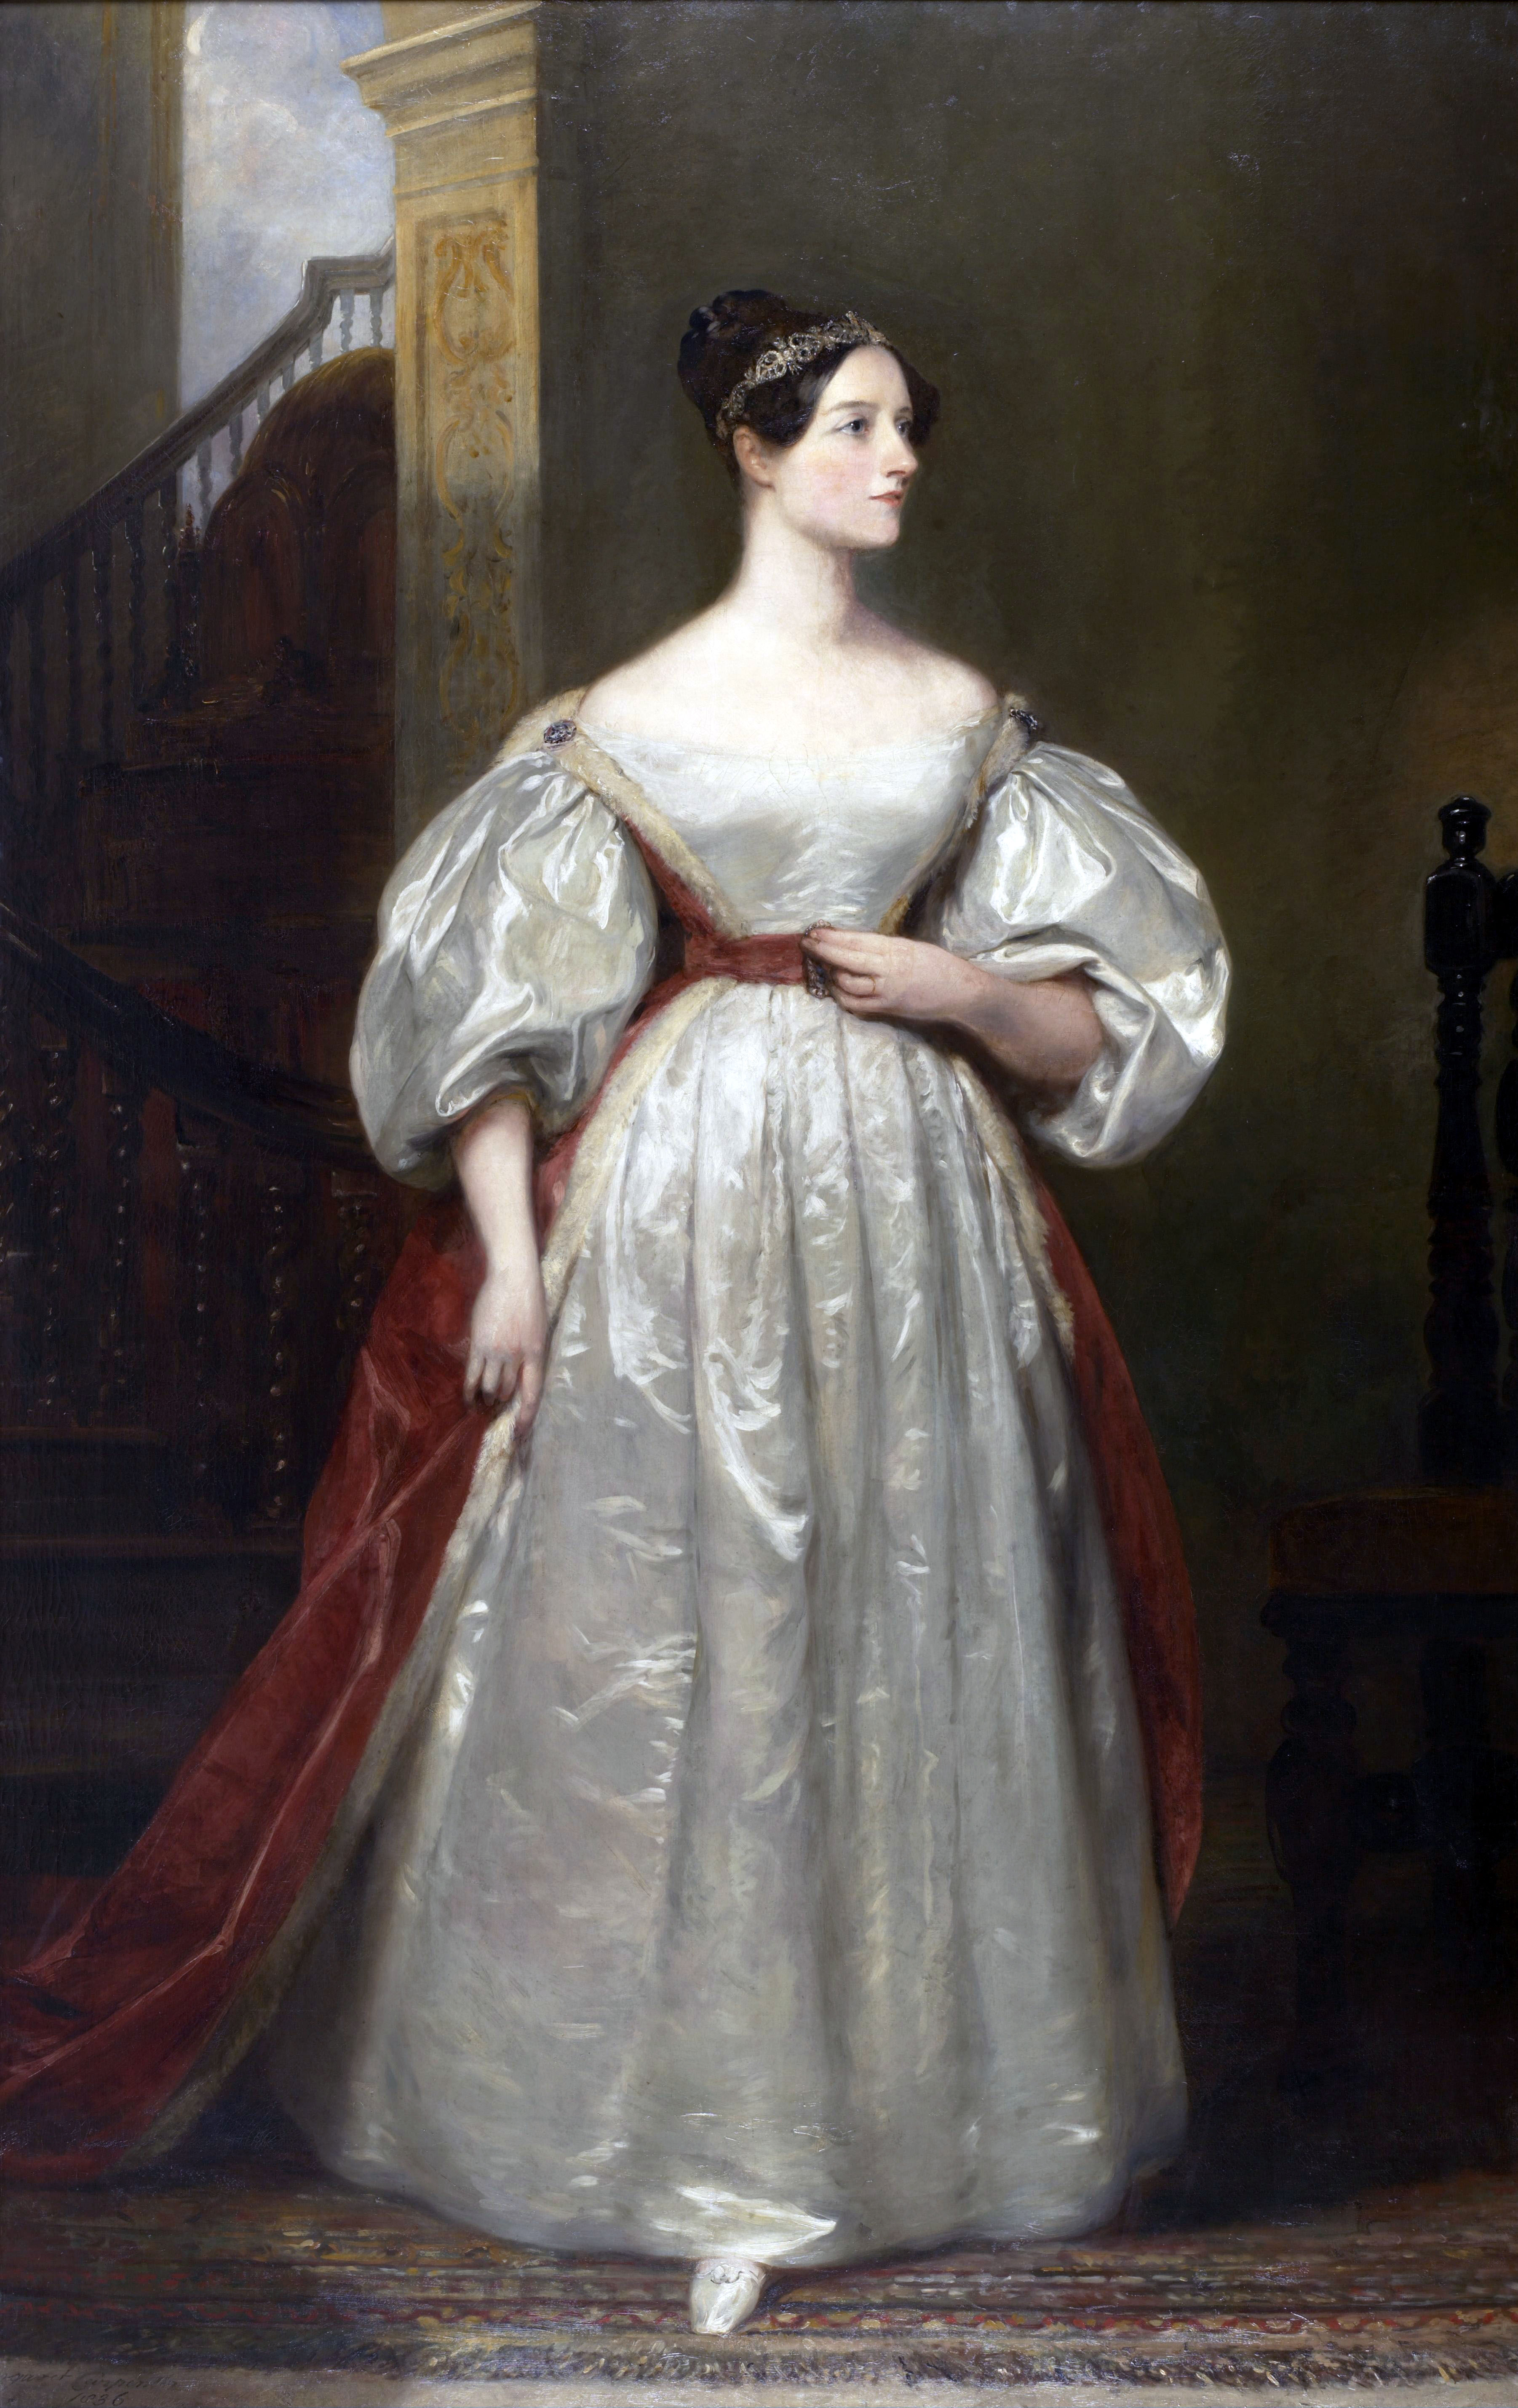
\includegraphics[width=0.725\linewidth]{./Images/Chapter00/ada-lovelace.jpg}\\ Ada \textsc{Lovelace}\\[10pt]
\textsc{Machine}\\[4pt]
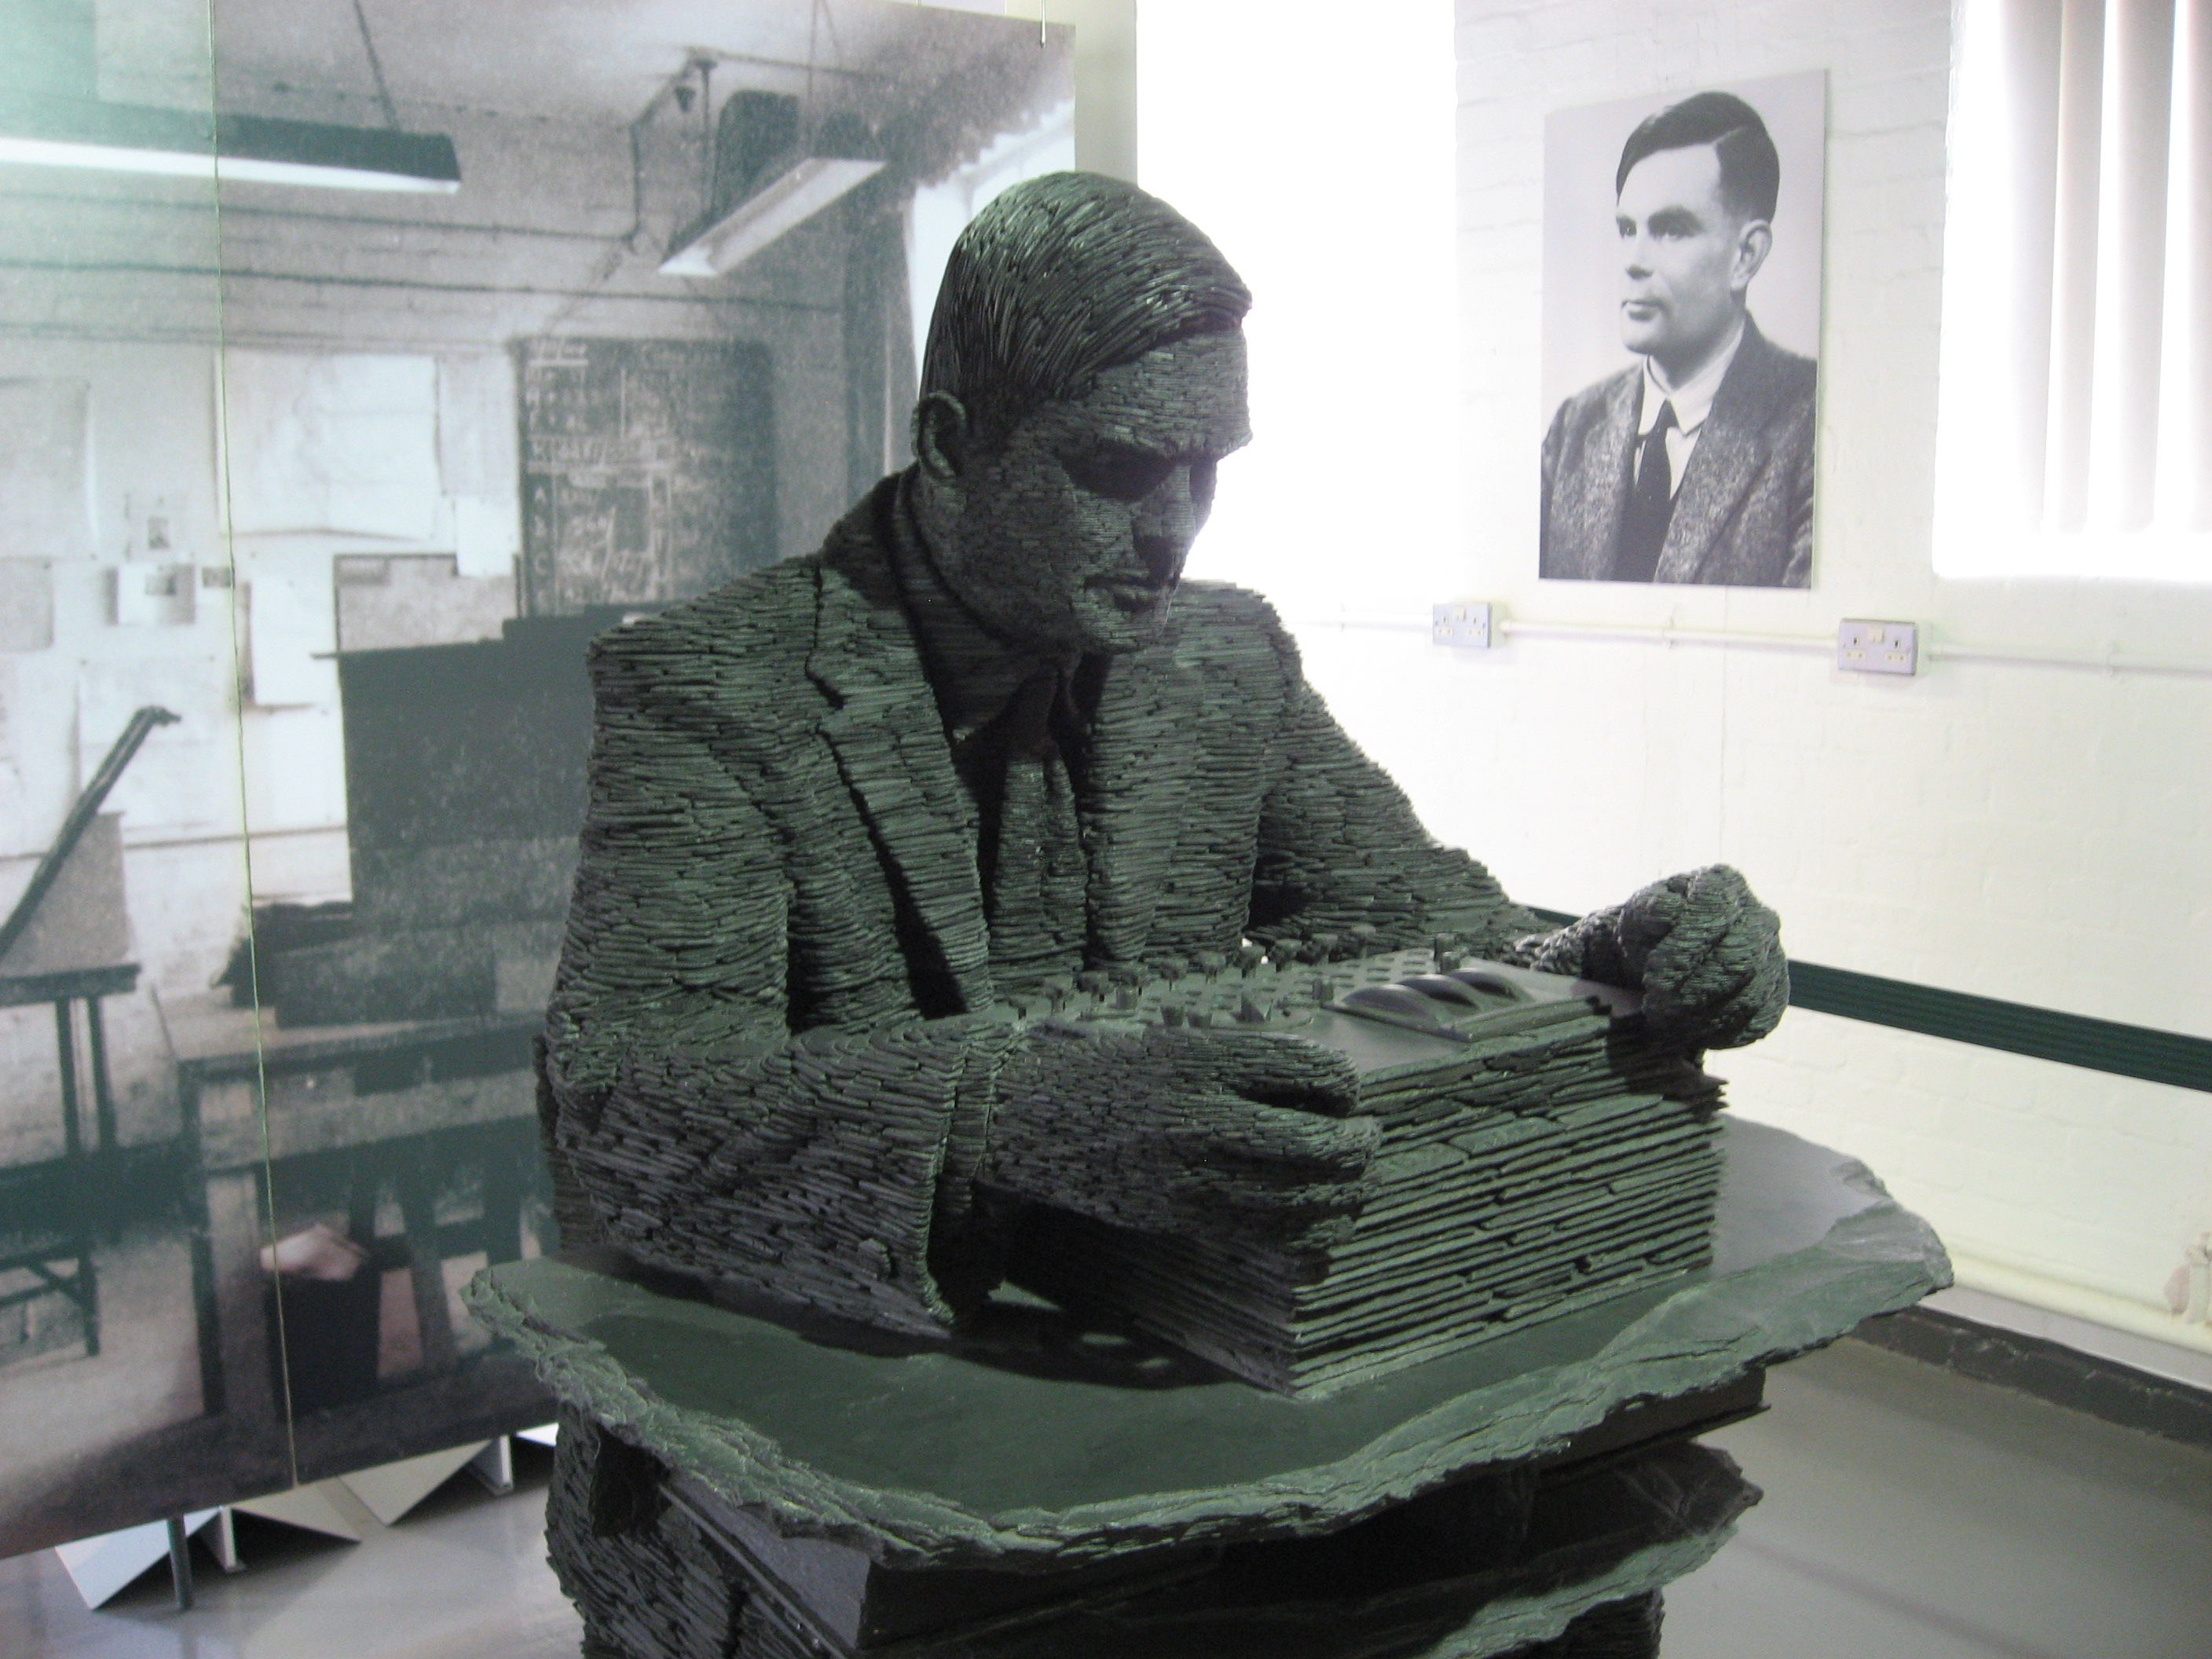
\includegraphics[width=0.725\linewidth]{./Images/Chapter00/alan-turing.jpg}\\ Alan \textsc{Turing}\\[10pt]
\textsc{Langage}\\[4pt]
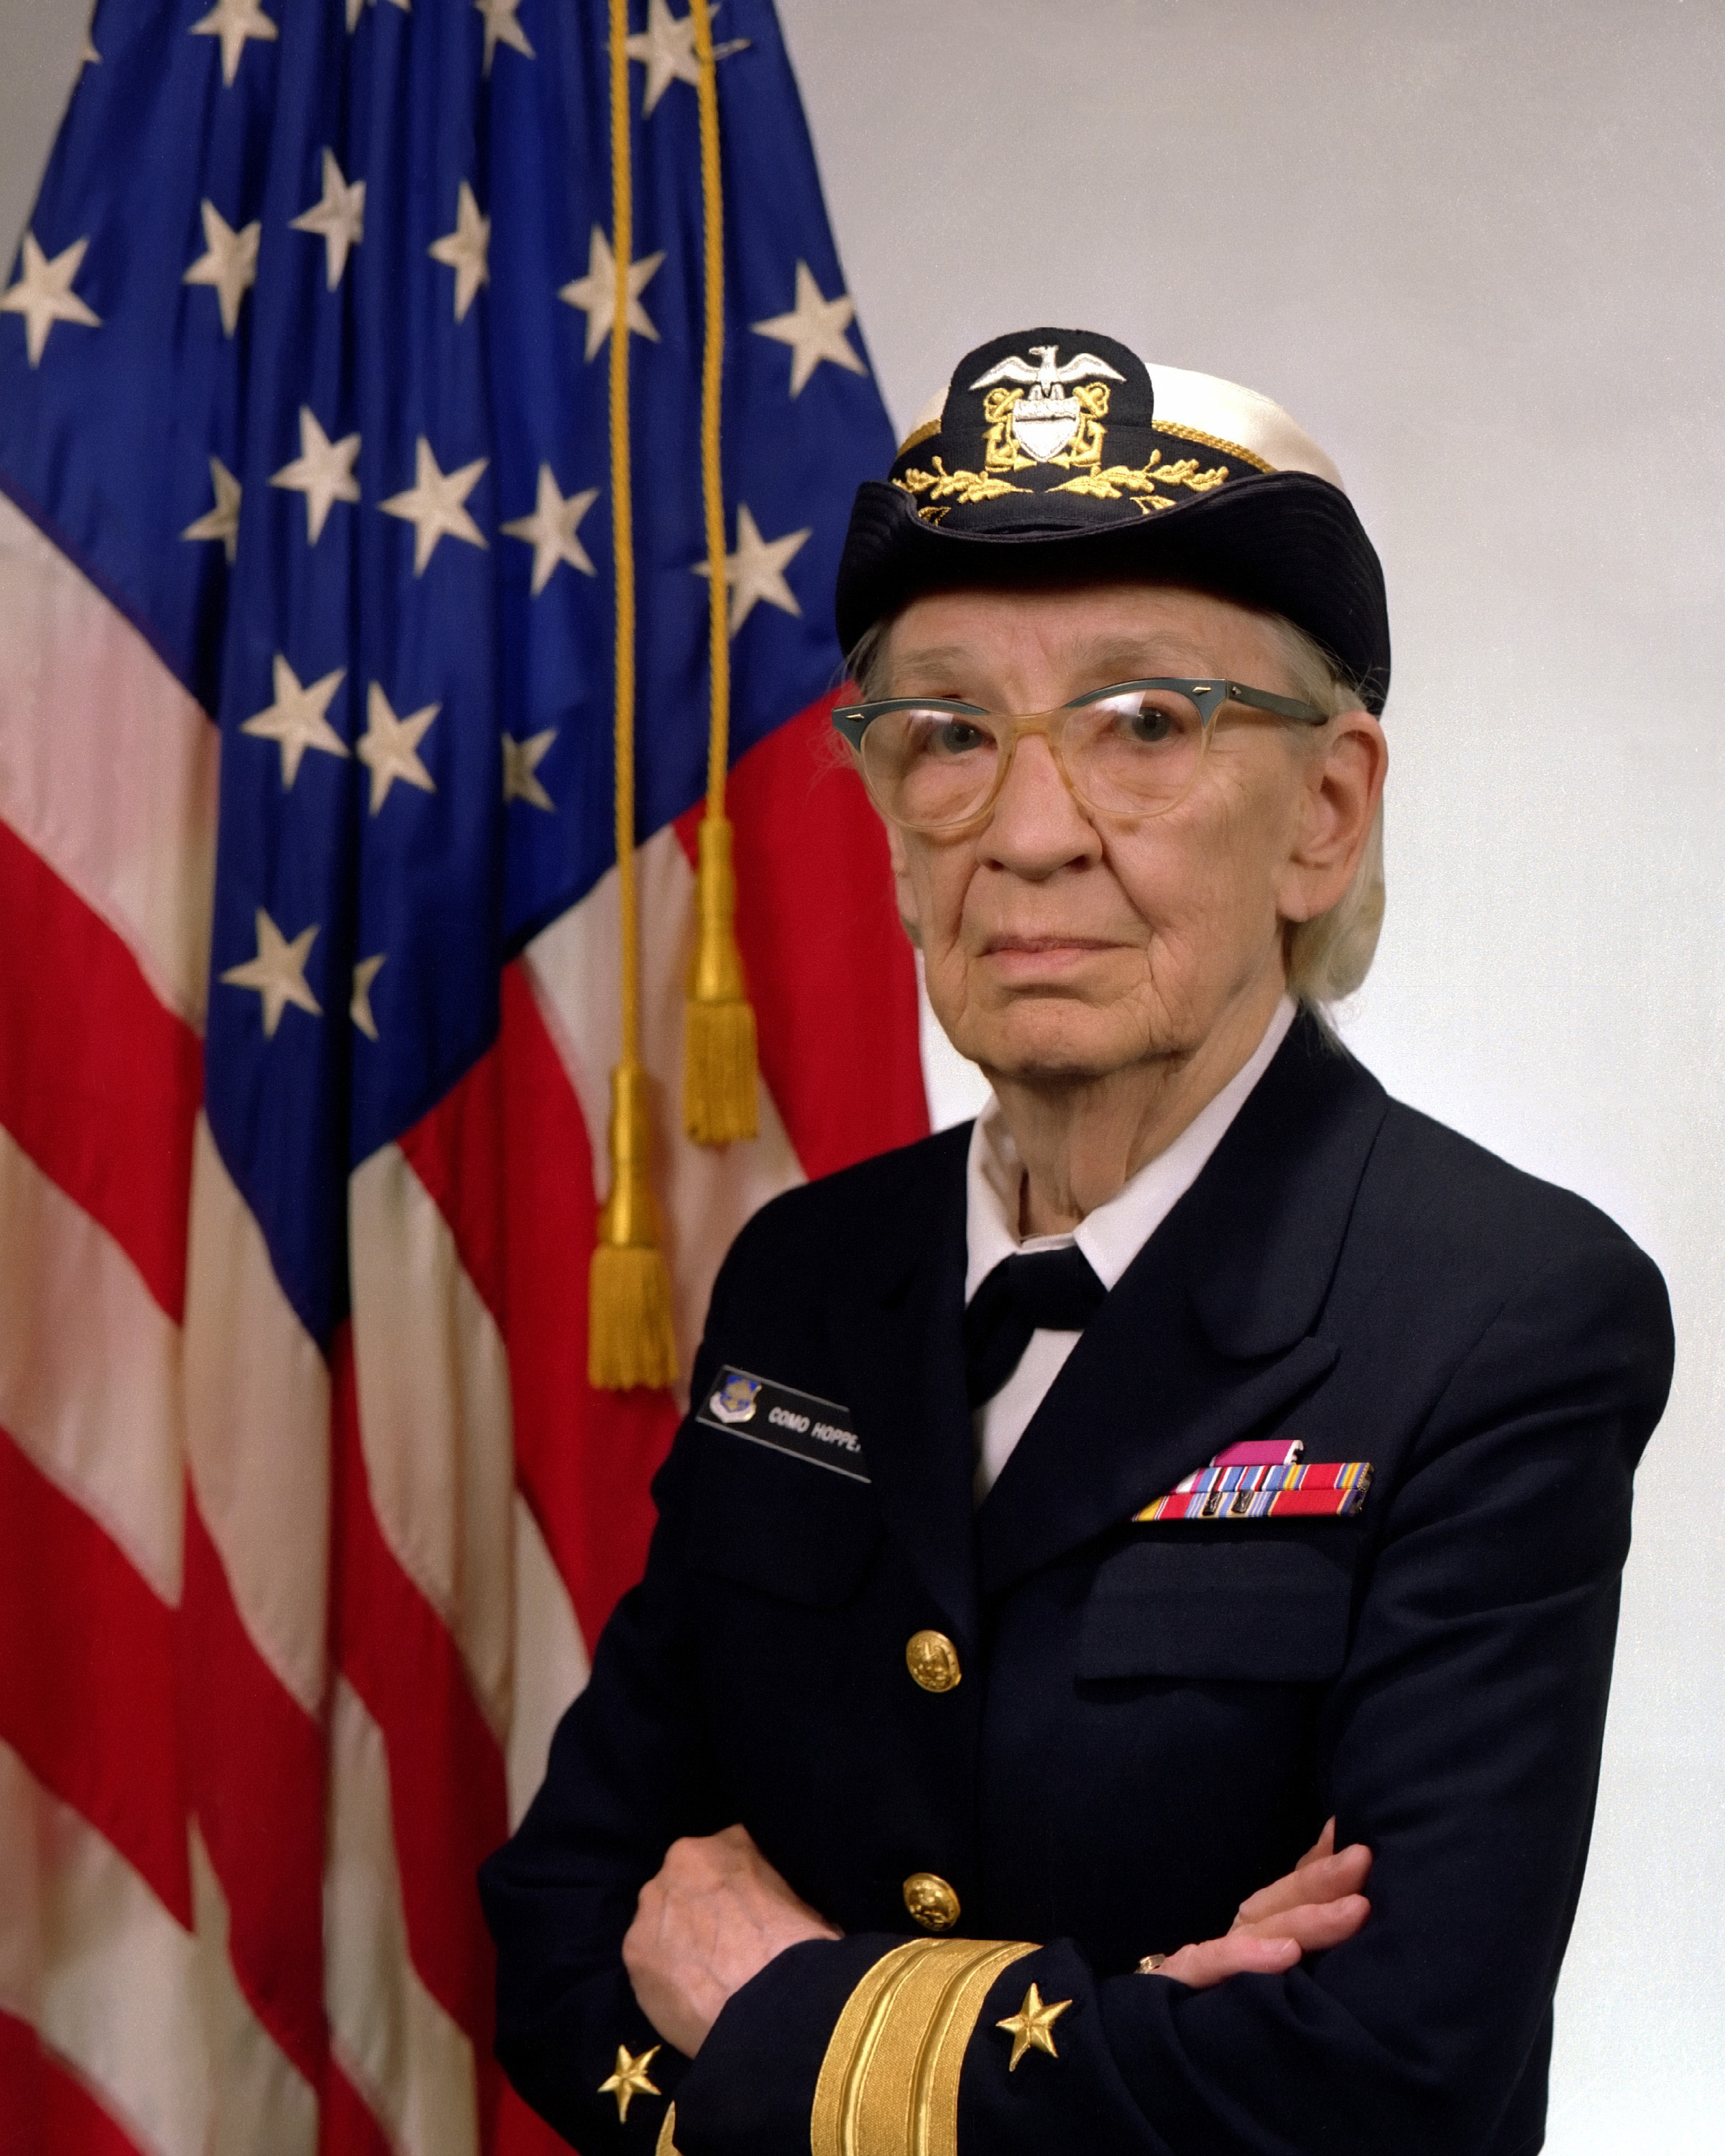
\includegraphics[width=0.725\linewidth]{./Images/Chapter00/grace-hopper.jpg}\\ Grace \textsc{Hopper}}{Wikimedia Commons}
Malgré leur grande variété, ces avancées se fondent toutes sur l’universalité et la flexibilité d’un petit nombre de concepts en interaction :
\begin{itemize}
	\item les \emph{données}, qui représentent sous une forme numérique unifiée des informations très diverses : textes, images, sons, mesures physiques, sommes d’argent, etc. ;
	\item les \emph{algorithmes}, qui spécifient de façon abstraite et précise des traitements à effectuer sur les données à partir d’opérations élémentaires ;
	\item les \emph{langages}, qui permettent de traduire les algorithmes abstraits en programmes textuels ou graphiques de façon à ce qu’ils soient exécutables par les machines ;
	\item les \emph{machines} et leurs systèmes d’exploitation, qui permettent d’exécuter des programmes, d'assurer le stockage des données et de gérer les communications, y compris les objets connectés et les réseaux.
\end{itemize}

À ces concepts s’ajoute un élément transversal : les interfaces qui permettent la communication avec les humains, la collecte des données et la commande des systèmes.


\subsection*{Motivation et attendus}

\overparagraph*{Compétences transversales}

Cet enseignement inclut l'acquisition :
\begin{itemize}
\item de savoirs (connaissance scientifique et technique en sciences [du] numérique[s]),
\item de savoir-faire (pratique de la programmation et de la création d'objets numériques),
\item et de savoir-être et agir pour savoir-devenir par rapport au numérique (attitude ni technophobe ni technophile, mais technocritique, au-delà des idées reçues pour tirer le meilleur du numérique et positionner son projet d'avenir face à cette réalité).
\end{itemize}

Au-delà, cet enseignement vise à développer \textit{deux grandes compétences transversales} : \textit{faire preuve d’autonomie, d’initiative et de créativité et développer sa réflexion personnelle et son esprit critique}.

\begin{center}
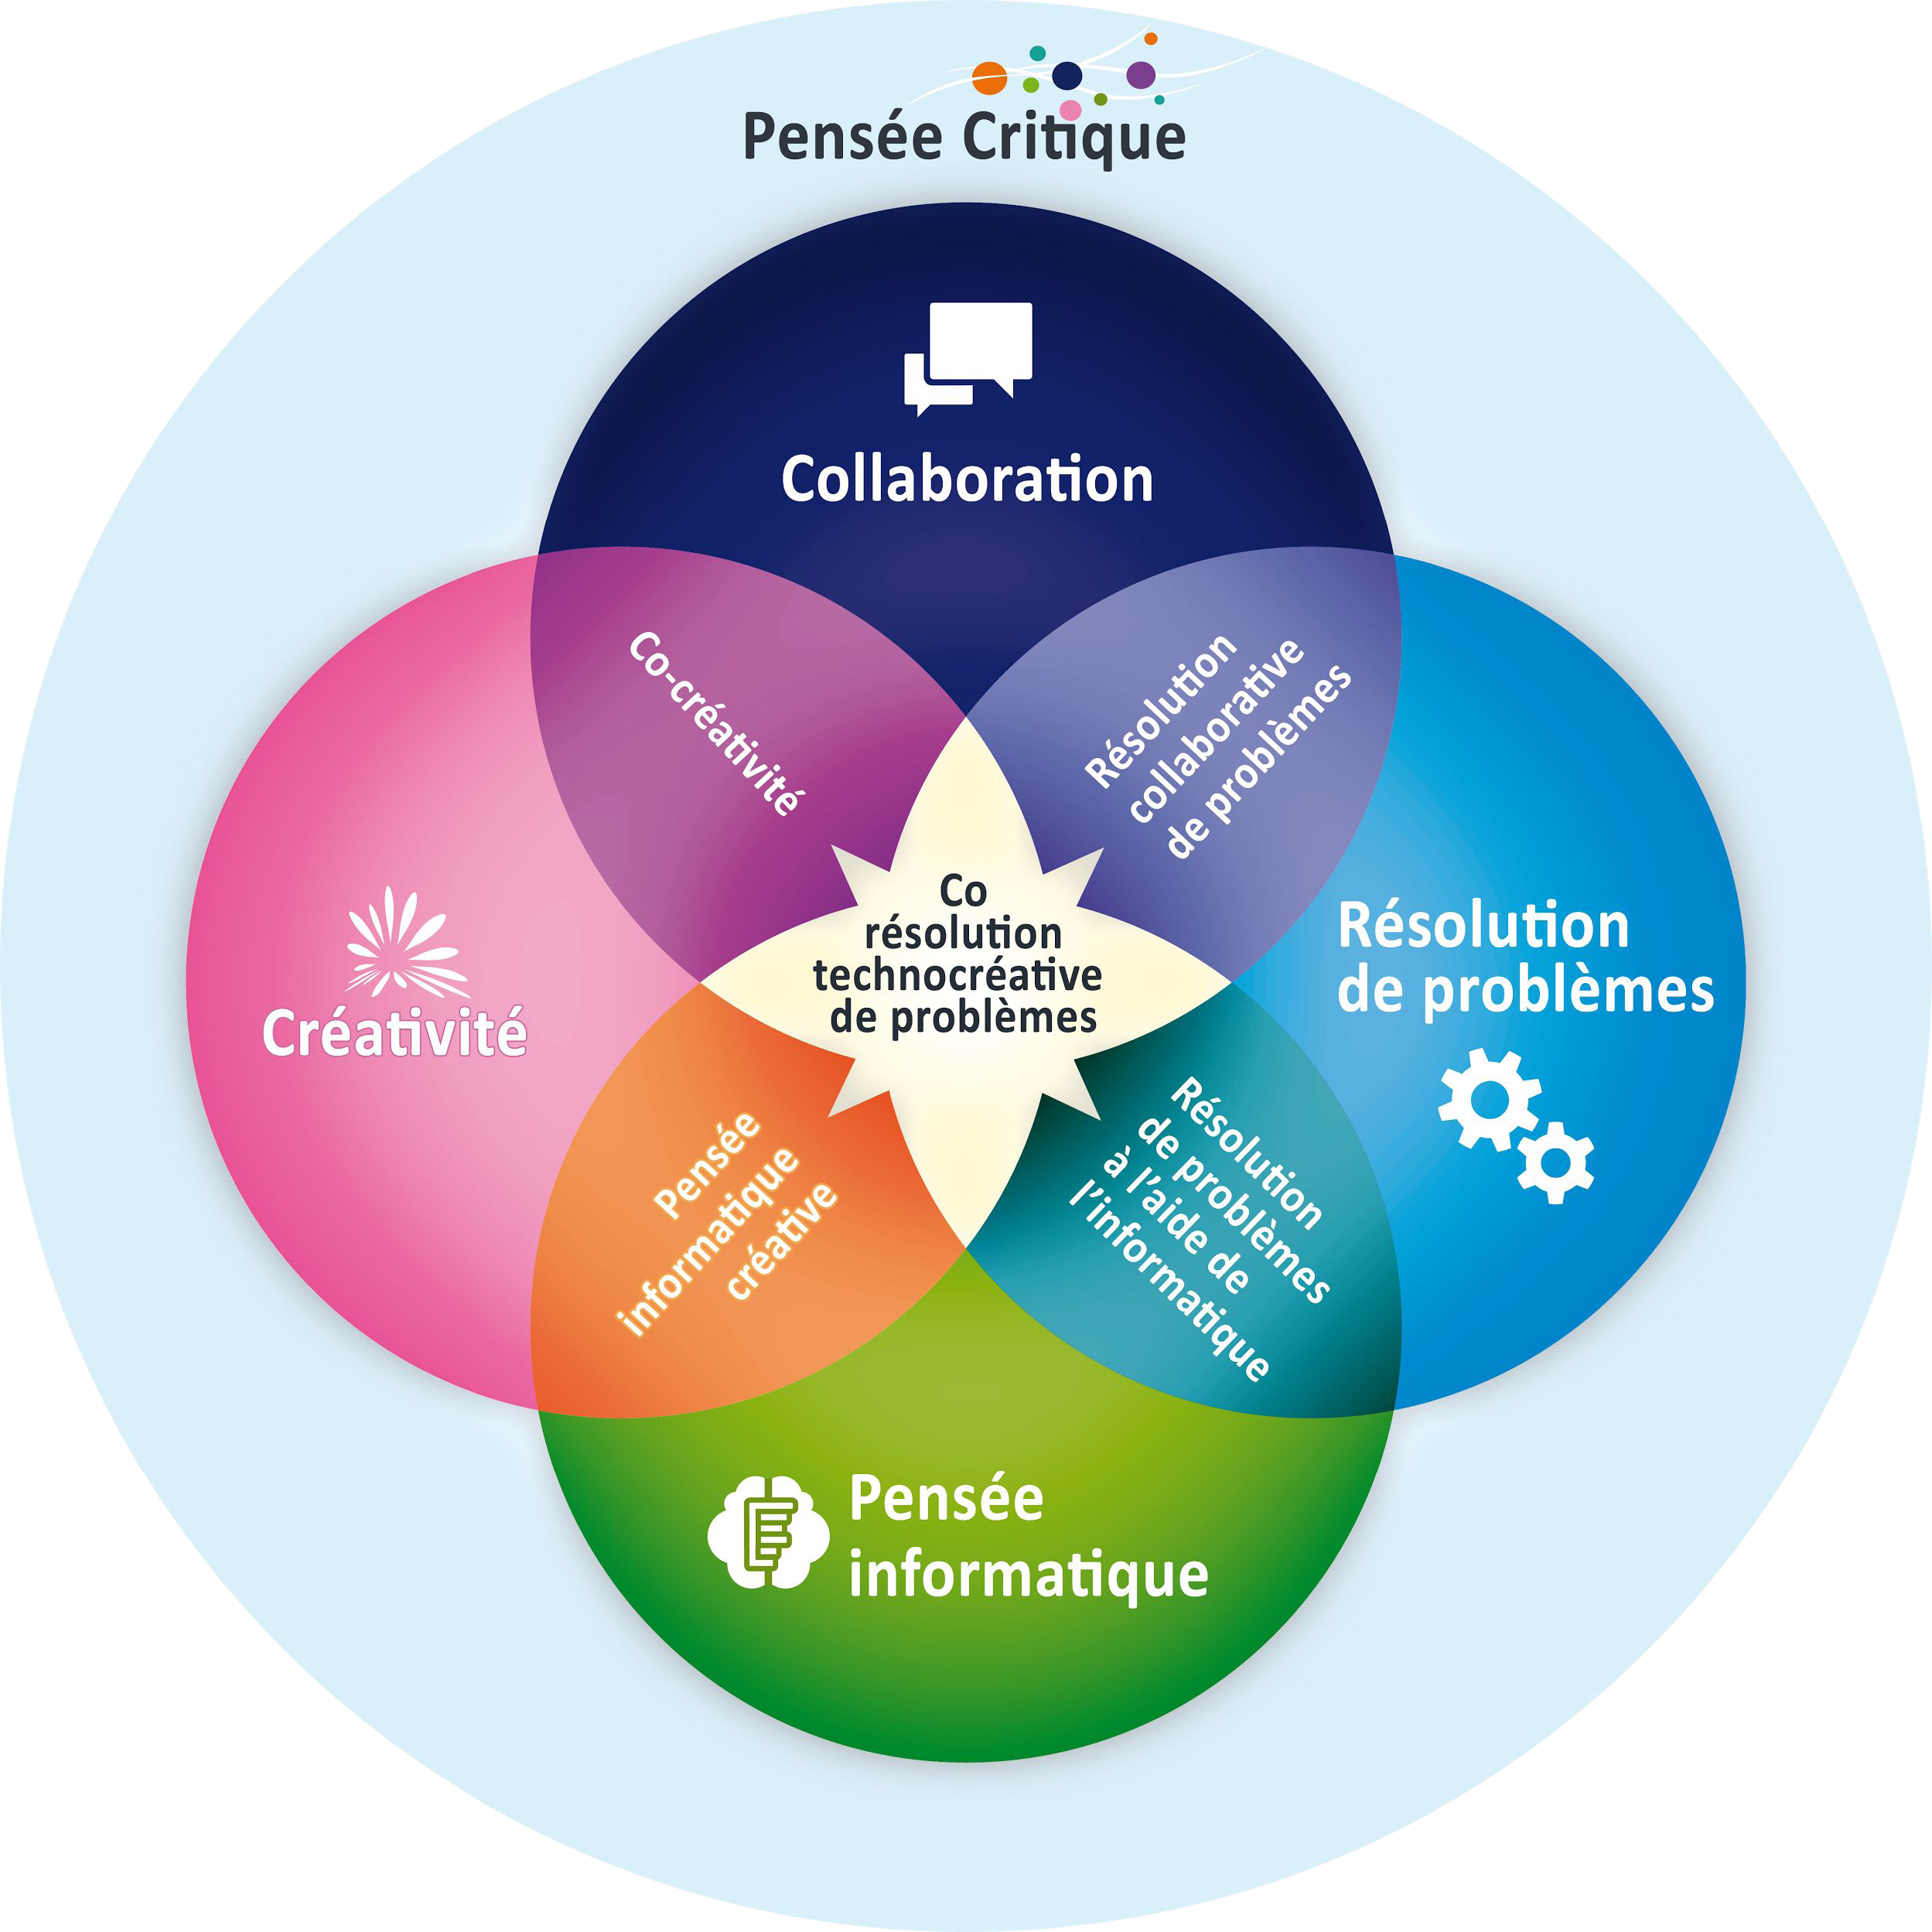
\includegraphics[width=0.8\linewidth]{./Images/Chapter00/cocreatic.png}
\end{center}

S'initier à la \href{https://project.inria.fr/classcode/mais-pourquoi-classcode-parle-de-pensee-informatique/}{pensée informatique} permet effectivement de développer les \href{https://en.wikipedia.org/wiki/21st_century_skills}{compétences du XXI\frup{e} siècle}, notamment la \href{https://pixees.fr/critique-de-lesprit-critique/}{pensée critique} et créative afin que tous les citoyens possèdent les connaissances minimales nécessaires à leur participation politique, économique, sociale et culturelle à l'ère du numérique, par exemple face à ce qu'on nomme intelligence artificielle.

Ces compétences font l'objet d'études et sont bien précisées, même si elles recouvrent des champs très vastes du développement de la personne en passe de devenir adulte. Elles sont aussi associées à des valeurs et à une vision humaniste du monde.

Apprendre à une future garagiste ou à un futur fleuriste, à programmer et à s'initier à la pensée informatique plutôt que de le ou la convaincre qu'il suffit de savoir utiliser les produits commerciaux du numérique, relève d'un vrai choix de société : celui de ne pas laisser les grands systèmes numériques être conçus par d'autres et de ne pas uniquement les consommer, voire les subir, mais participer à leur création et se donner les moyens d'en user de manière critique.

%Regardons en deux figures et une lecture (dans l'onglet suivant), de quoi il s'agit.

%De quoi s'agit-il (voir illustrations) ?

\overparagraph*{Compétences, attitudes et valeurs}

\sidegraphic{
\includegraphics[width=\linewidth]{./Images/Chapter00/eduscol.png}}
On liste ici les mots-clés qui permettent de relier les grands éléments de ces compétences transversales à des notions usuelles que nous connaissons bien et qui s'intègrent naturellement dans nos démarches pédagogiques.

\begin{fullwidth}
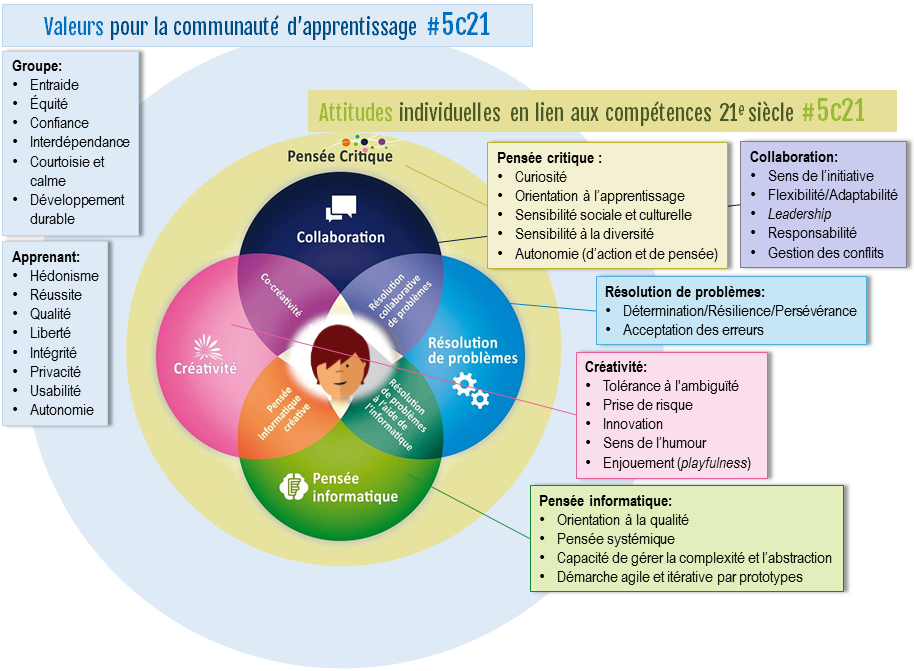
\includegraphics[width=\linewidth]{./Images/Chapter00/cocreatic-comment.png}
\end{fullwidth}

%\vfill

\overparagraph*{Développer l'esprit critique}

L’\href{https://fr.wikipedia.org/wiki/Esprit_critique}{esprit critique} est une démarche de questionnement des opinions ou des théories, mais aussi une posture intellectuelle humaniste : je m’intéresse aux arguments utilisés par l'autre, à ce qui conduit à les exprimer (voir par exemple cette \href{https://pixees.fr/critique-de-lesprit-critique/}{critique de l'esprit critique}).


\begin{fullwidth}
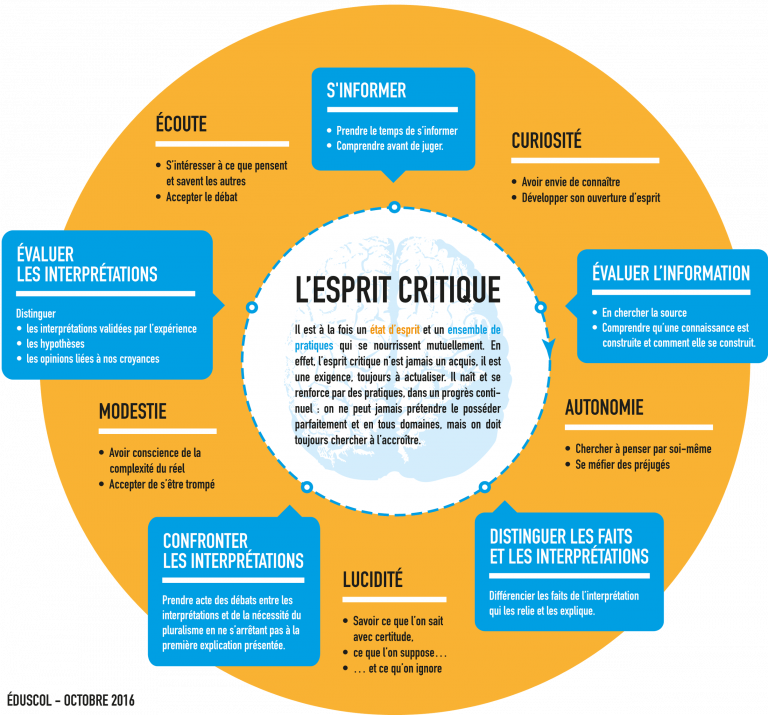
\includegraphics[width=\linewidth]{./Images/Chapter00/critique-esprit-critique.png}
\end{fullwidth}


\subsection*{Savoirs informatiques}

\overparagraph*{Pensée informatique}

\sidegraphic{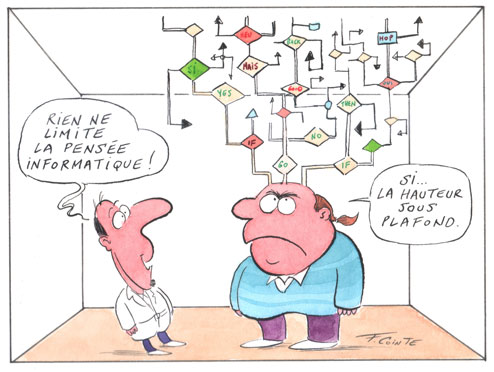
\includegraphics[width=\linewidth]{./Images/Chapter00/pensee-informatique.png}}{François Cointe}
La \href{https://interstices.info/la-pensee-informatique/}{pensée informatique} a une définition, due à \href{https://fr.wikipedia.org/wiki/Jeannette_Wing}{Jeannette \textsc{Wing}}. C’est un ensemble de compétences et de connaissances, utilisées en science et technologie informatique, mais applicables à d’autres domaines.

Cette panoplie d’outils intellectuels inclut, par exemple, la capacité à nommer de manière pertinente les objets et en expliciter leur type ou catégorie pour les manipuler correctement, à maîtriser la complexité d’un grand problème ou d’un système en le hiérarchisant, à pouvoir spécifier dans ses moindres détails un procédé pour qu’il puisse s’exécuter sans ambiguïté de manière mécanique, etc.

En résumé, \href{https://project.inria.fr/classcode/mais-pourquoi-classcode-parle-de-pensee-informatique/}{l’informatique ne sert pas qu’en informatique} comme discuté au niveau du projet \textsc{Class´Code} qui a produit cette formation et comme détaillé dans l'\href{https://interstices.info/la-pensee-informatique/}{article originel} de \href{https://interstices.info/auteur/jeannette-wing/}{Jeannette \textsc{Wing}}. Peut-on définir un mode de pensée spécifique à l'informatique ? La pensée informatique est présentée ici comme un ensemble d'attitudes et de connaissances universellement applicables, que nous gagnerions tous à apprendre et à maîtriser.

\begin{fullwidth}
% Image : https://pixabay.com/fr/photos/intelligence-artificielle-cerveau-3382521/
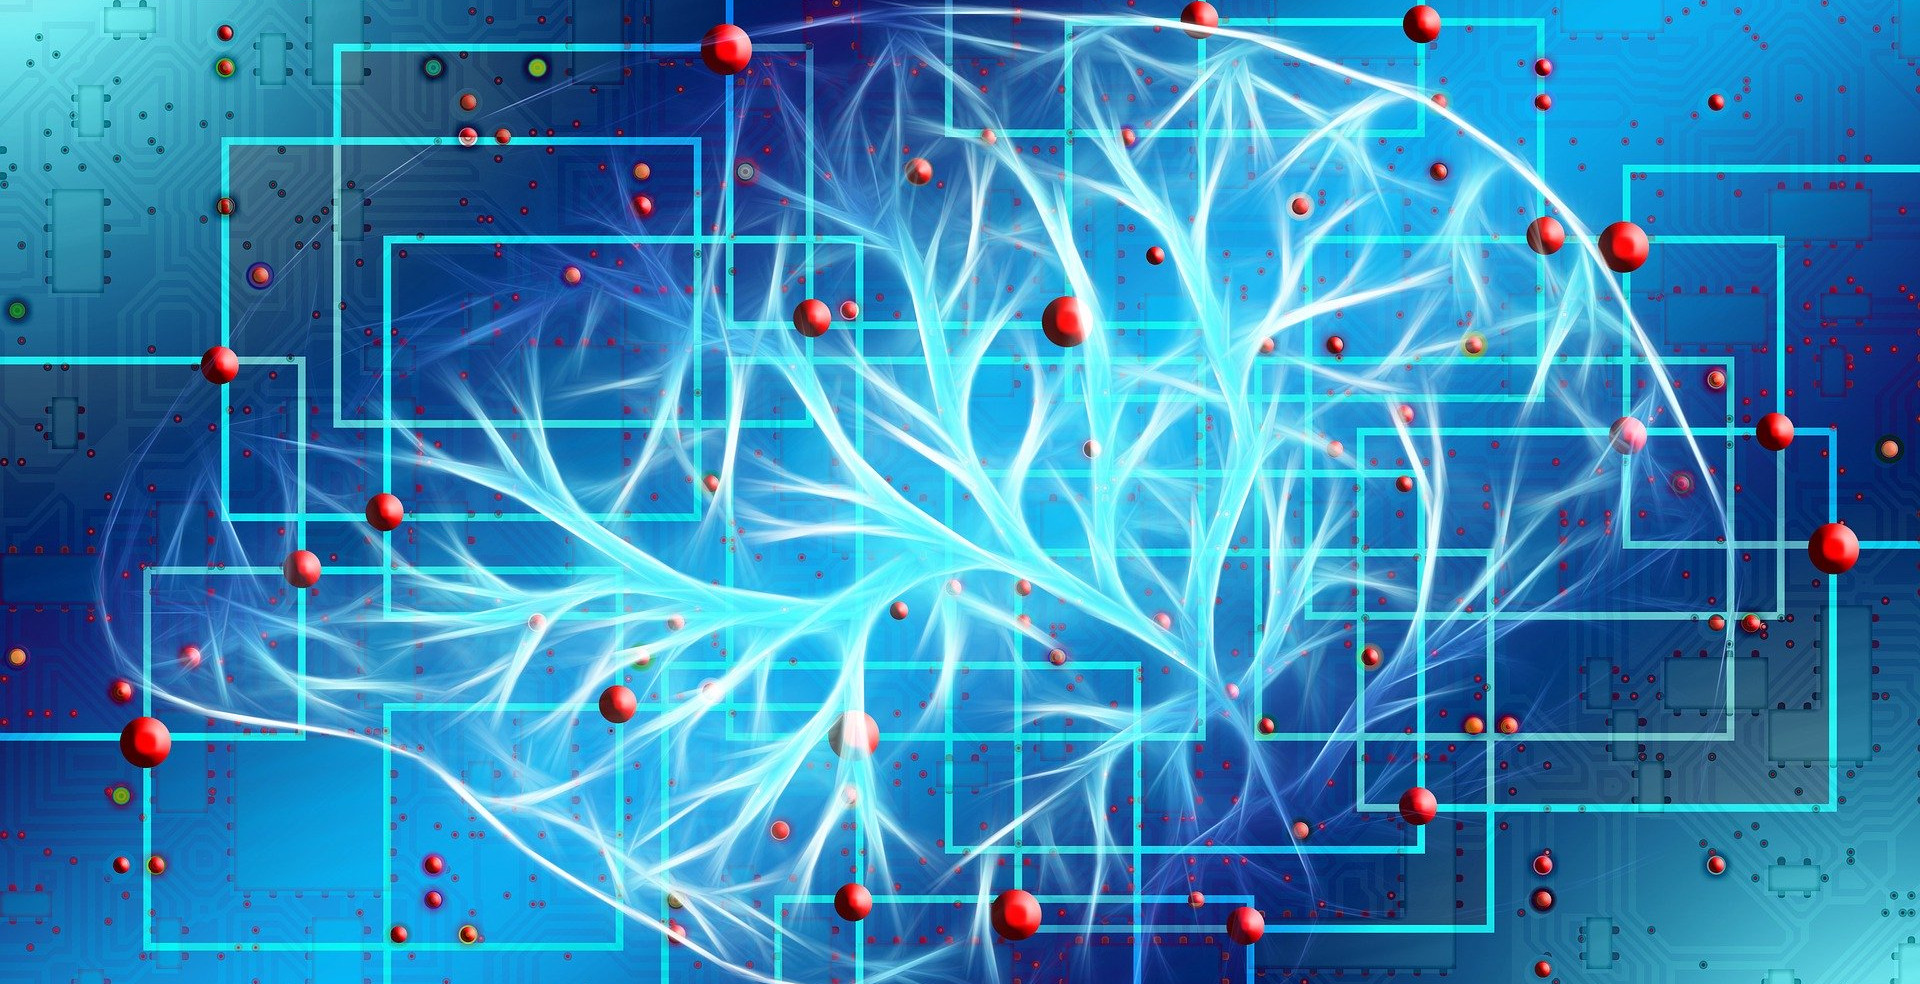
\includegraphics[width=\linewidth]{./Images/Chapter00/ai-gerd-altmann.jpg}
\llap{%
\begin{tikzpicture}[remember picture, overlay]
\node[anchor=west, inner sep=0pt, rotate=90, xshift=10pt, yshift=6pt] at (0,0) {\scriptsize\faCopyright\space Gerd Altmann via Pixabay};
\end{tikzpicture}%
}
\end{fullwidth}

\overparagraph*{Enseignement de l'informatique}

\begin{marginvideo*}[\label{vid:0.1}Éducation à l'informatique.]%
	\movie[width=\marginparwidth,showcontrols]%
		{
\includegraphics[width=\marginparwidth]{./Images/Pictograms/film-strip-dark-electric-blue.png}}%
		{https://www.college-de-france.fr/video/gerard-berry/2008/berry-20080117.mp4}%
	%\launchvideo{./Videos/Chapter00/berry-2019-02-06.mp4}
	\launchvideo{https://www.college-de-france.fr/site/gerard-berry/inaugural-lecture-2008-01-17-18h00.htm}
\end{marginvideo*}

%\sidegraphic{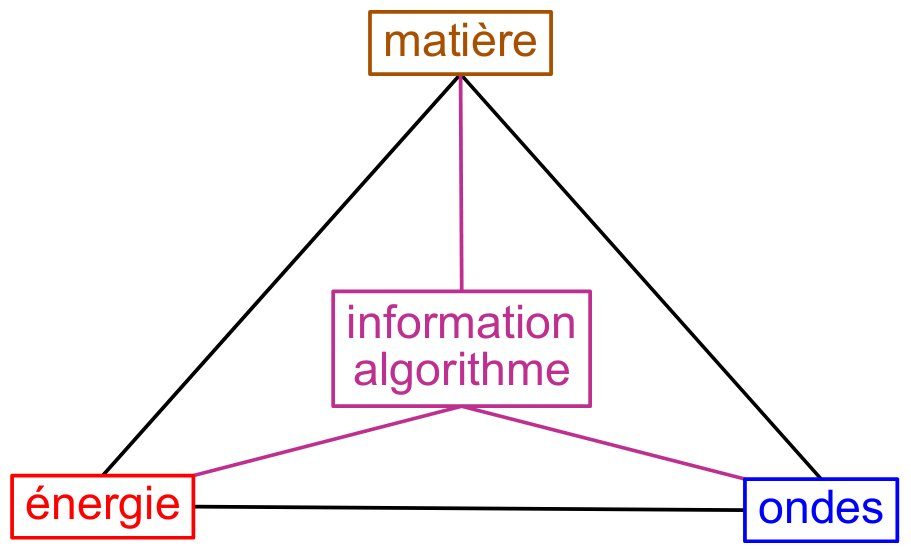
\includegraphics[width=\linewidth]{./Images/Chapter00/information_et_monde_physique.jpg}}
\blockquotation[Gérard \textsc{Berry}]{%
L’information ne pèse pas, ne brûle pas, ne sent pas, ce n'est pas une quantité physique usuelle, et pourtant elle se stocke, se transporte et se duplique très facilement, tandis qu'elle se transforme avec des algorithmes. Cela conduit à une nouvelle façon de penser et d’agir avec des leviers d’une immense efficacité.}

En février 2019, Gérard \textsc{Berry} fait le point sur l'enseignement --- et l'éducation --- à l'informatique, lors d'un cours au Collège de France (à \href{./Videos/Chapter00/berry-2019-02-06.mp4}{visionner}, durée 1h15mn et/ou à consulter les \href{https://www.college-de-france.fr/media/gerard-berry/UPL7003896140239979456_2019_02_06_Berry_Cours3_EnseignementInfo.pdf}{planches de diaporama}).

\begin{graphic}
%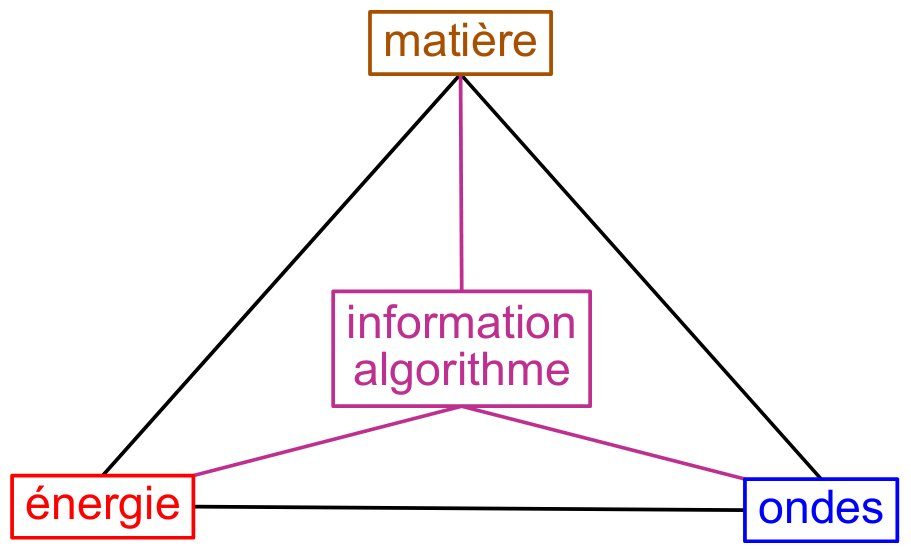
\includegraphics[width=0.4\linewidth]{./Images/Chapter00/information_et_monde_physique.jpg}
\centering
\begin{tikzpicture}
%\draw[step=0.25cm,style=help lines, line width=0.1pt] (-5,-2.75) grid (5,2.75);
%\draw[step=1cm,style=help lines, line width=0.8pt] (-5,-2.75) grid (5,2.75);
\node[draw, very thick, firstcolor] (matter) at (0,2.25) {\strut Matière};
\node[draw, very thick, secondcolor] (information) at (0,-0.5) {\begin{tabular}{@{}c@{}}Information\\ Algorithme\end{tabular}};
\node[draw, very thick, firstcolor] (energy) at (-4.0,-2.25) {\strut Énergie};
\node[draw, very thick, firstcolor] (waves) at (4.0,-2.25) {\strut Ondes};
\draw[ultra thick, firstcolor, latex-latex] (matter.south) -- node[midway, left, font=\small, xshift=-4pt, firstcolor]{Début XIX\frup{e} siècle} (energy.north);
\draw[ultra thick, firstcolor, latex-latex] (matter.south) -- node[midway, right, font=\small, xshift=4pt, firstcolor]{Milieu XIX\frup{e} siècle} (waves.north);
\draw[ultra thick, firstcolor, latex-latex] (energy.east) -- (waves.west);
\node[font=\small, yshift=0pt, firstcolor] at (0,-2.5) {Début XX\frup{e} siècle};
\draw[ultra thick, secondcolor, latex-latex] (information.south) -- (energy.north east);
\draw[ultra thick, secondcolor, latex-latex] (information.south) -- (waves.north west);
\draw[ultra thick, secondcolor, latex-latex] (information.north) -- (matter.south);
\node[font=\small, yshift=4pt, secondcolor] at (0,-1.75) {XX\frup{e} et XXI\frup{e} siècles};
\end{tikzpicture}
\vspace{4pt}
\caption{\label{graph:01}Information et monde physique : évolution des sciences et techniques.}
\end{graphic}


%\vfill\pagebreak

\subsection*{Ouvrages généraux de référence}

\begin{description}
\item[Informatique et sciences du numérique] --- 
\sidegraphic{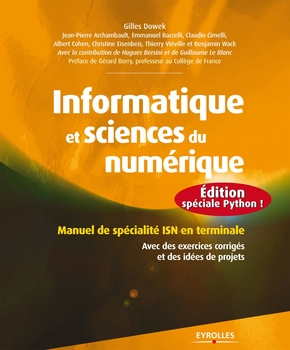
\includegraphics[scale=0.25]{./Images/Chapter00/dowek-etal-2013.jpg}\\ \footnotesize\parencite{Dowek-etal:2013}} 
Gilles \textsc{Dowek} et al. (352 pp, Eyrolles éditeur,  août 2013). Ce manuel librement accessible en ligne, est le manuel de spécialité ISN en terminale, avec des exercices corrigés et des idées de projets, il contient toutes les notions de base dont on a besoin en SNT pour se former, et beaucoup d'éléments pour préparer les cours, en faisant attention aux éléments hors programme.
\item[Enseigner l'informatique] --- 
\sidegraphic{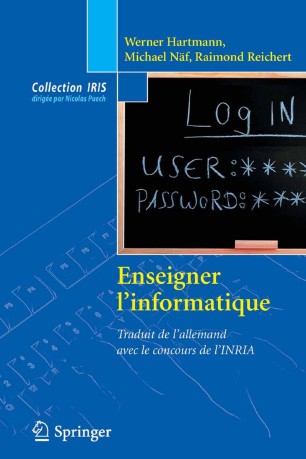
\includegraphics[scale=0.2]{./Images/Chapter00/hartmann-etal-2011.jpeg}\\ \footnotesize\parencite{Hartmann-etal:2011}} 
Werner \textsc{Hartmann Werner}, Michael \textsc{Näf}, \linebreak Raimond \textsc{Reichert} avec Robert \textsc{Cabane} (176 pp, Springer Verlag, Collection Iris, 2011). Explique ce qu’un enseignement de l’informatique doit être, ce qu’il n’est pas et ce qu’il ne doit surtout pas devenir. Il explore méthodiquement certaines questions avec des situations vécues quotidiennement au nombre desquelles : existe-t-il une didactique de l’informatique ? Une pédagogie vaut-elle mieux qu’une autre ? Comment gérer la diversité au sein des groupes qui apprennent l’informatique ? Pourquoi et comment aborder l’abstraction ?
\item[Le temps des algorithmes] --- 
\sidegraphic{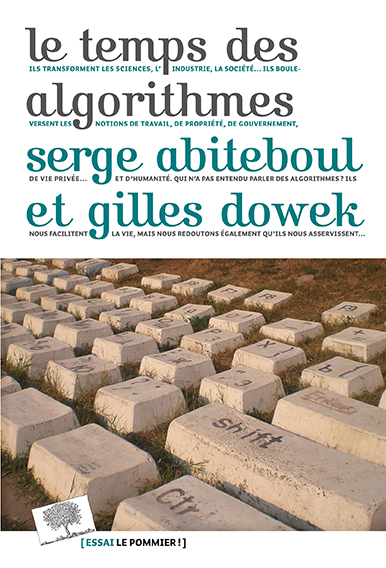
\includegraphics[scale=0.125]{./Images/Chapter00/abitboul-dowek-2017.jpg}\\ \footnotesize\parencite{Abitboul-Dowek:2017}} 
Serge \textsc{Abiteboul} et Gilles \textsc{Dowek} (192 pp,  Éditions le Pommier, Collection Essais, janvier 2017). Cet ouvrage nous aide à nous poser des questions fondamentales sur la place des algorithmes dans notre société, où les relations sociales, la vie professionnelle, la propriété des biens immatériels, médecine, industrie, transport, sciences jusqu’à la démocratie même, subissent de vrais bouleversements. Il permet de prendre du recul par rapport aux aspects sociétaux du programme et de les nourrir des liens avec la science et technologie informatique.
\item[Histoire illustrée de l'informatique] --- 
\sidegraphic{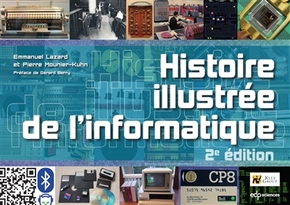
\includegraphics[scale=0.25]{./Images/Chapter00/lazard-mounier-kuhn-2016.jpg}\\ \footnotesize\parencite{Lazar-Mounier:2019}} 
Emmanuel \textsc{Lazard} et Pierre-Éric \textsc{Mounier-Kuhn} (240 pp, EDP Sciences, 2019). Une description de l’histoire de l’informatique et du numérique à travers des dates et des événements concrets (Antiquité, XVII\frup{e} au XIX\frup{e} siècle et surtout XX\frup{e} et XXI\frup{e} siècles). Une base de connaissances de référence pour préparer ces cours et fournir de repères au élèves.
\item[Apprentissages et documents numériques] --- 
\sidegraphic{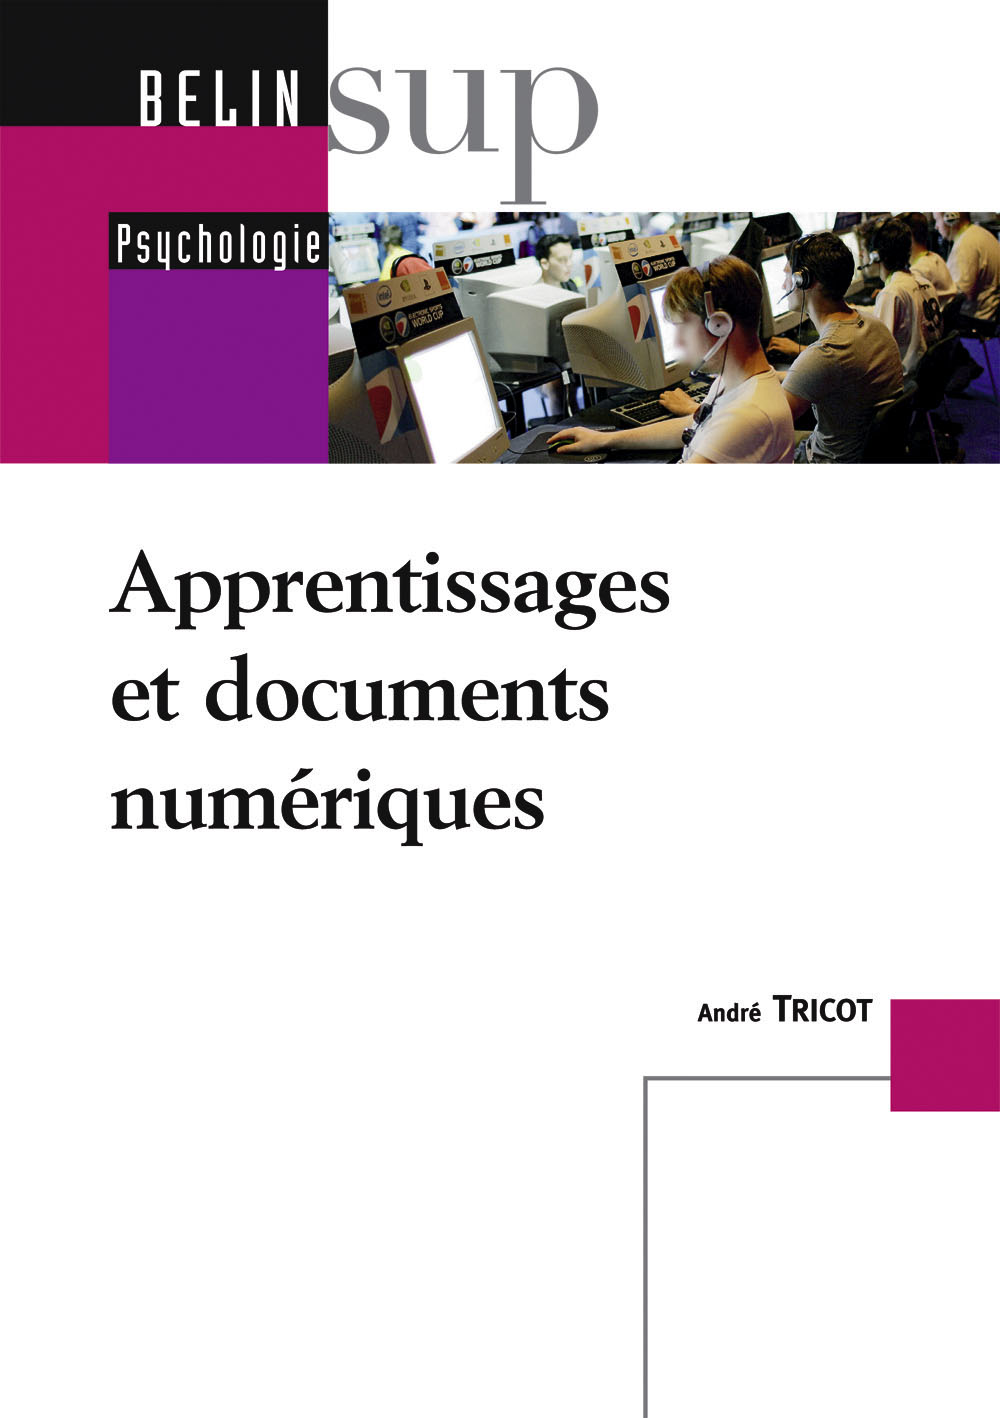
\includegraphics[scale=0.225]{./Images/Chapter00/tricot-2007.jpg}\\ \footnotesize\parencite{Tricot:2007}} 
André \textsc{Tricot} (277 pp, Éditions Belin, Sup psychologie, 2007). Chaque idée relativement à l'apprentissage avec des documents et outils numériques est passée au crible avec une méthode simple et rigoureuse : énoncer un mythe (par exemple le mythe de l’apprentissage ludique) et préciser en quoi il consiste. Étudier ce qu’en disent les travaux scientifiques. Donner des exemples (de jeux sérieux, dans le chapitre cité). Et en tirer une conclusion, sérieuse, modérée et sans prétention. Voir aussi deux ouvrages complémentaires plus récents : \href{http://www.cafepedagogique.net/lexpresso/Pages/2014/10/21102014Article635494737667005194.aspx}{Apprendre avec le numérique} et \href{http://www.cafepedagogique.net/LEXPRESSO/Pages/2017/09/05092017Article636401937485284884.aspx}{L'innovation pédagogique}.
\item[Au cœur des réseaux : des sciences aux citoyens] --- 
\sidegraphic{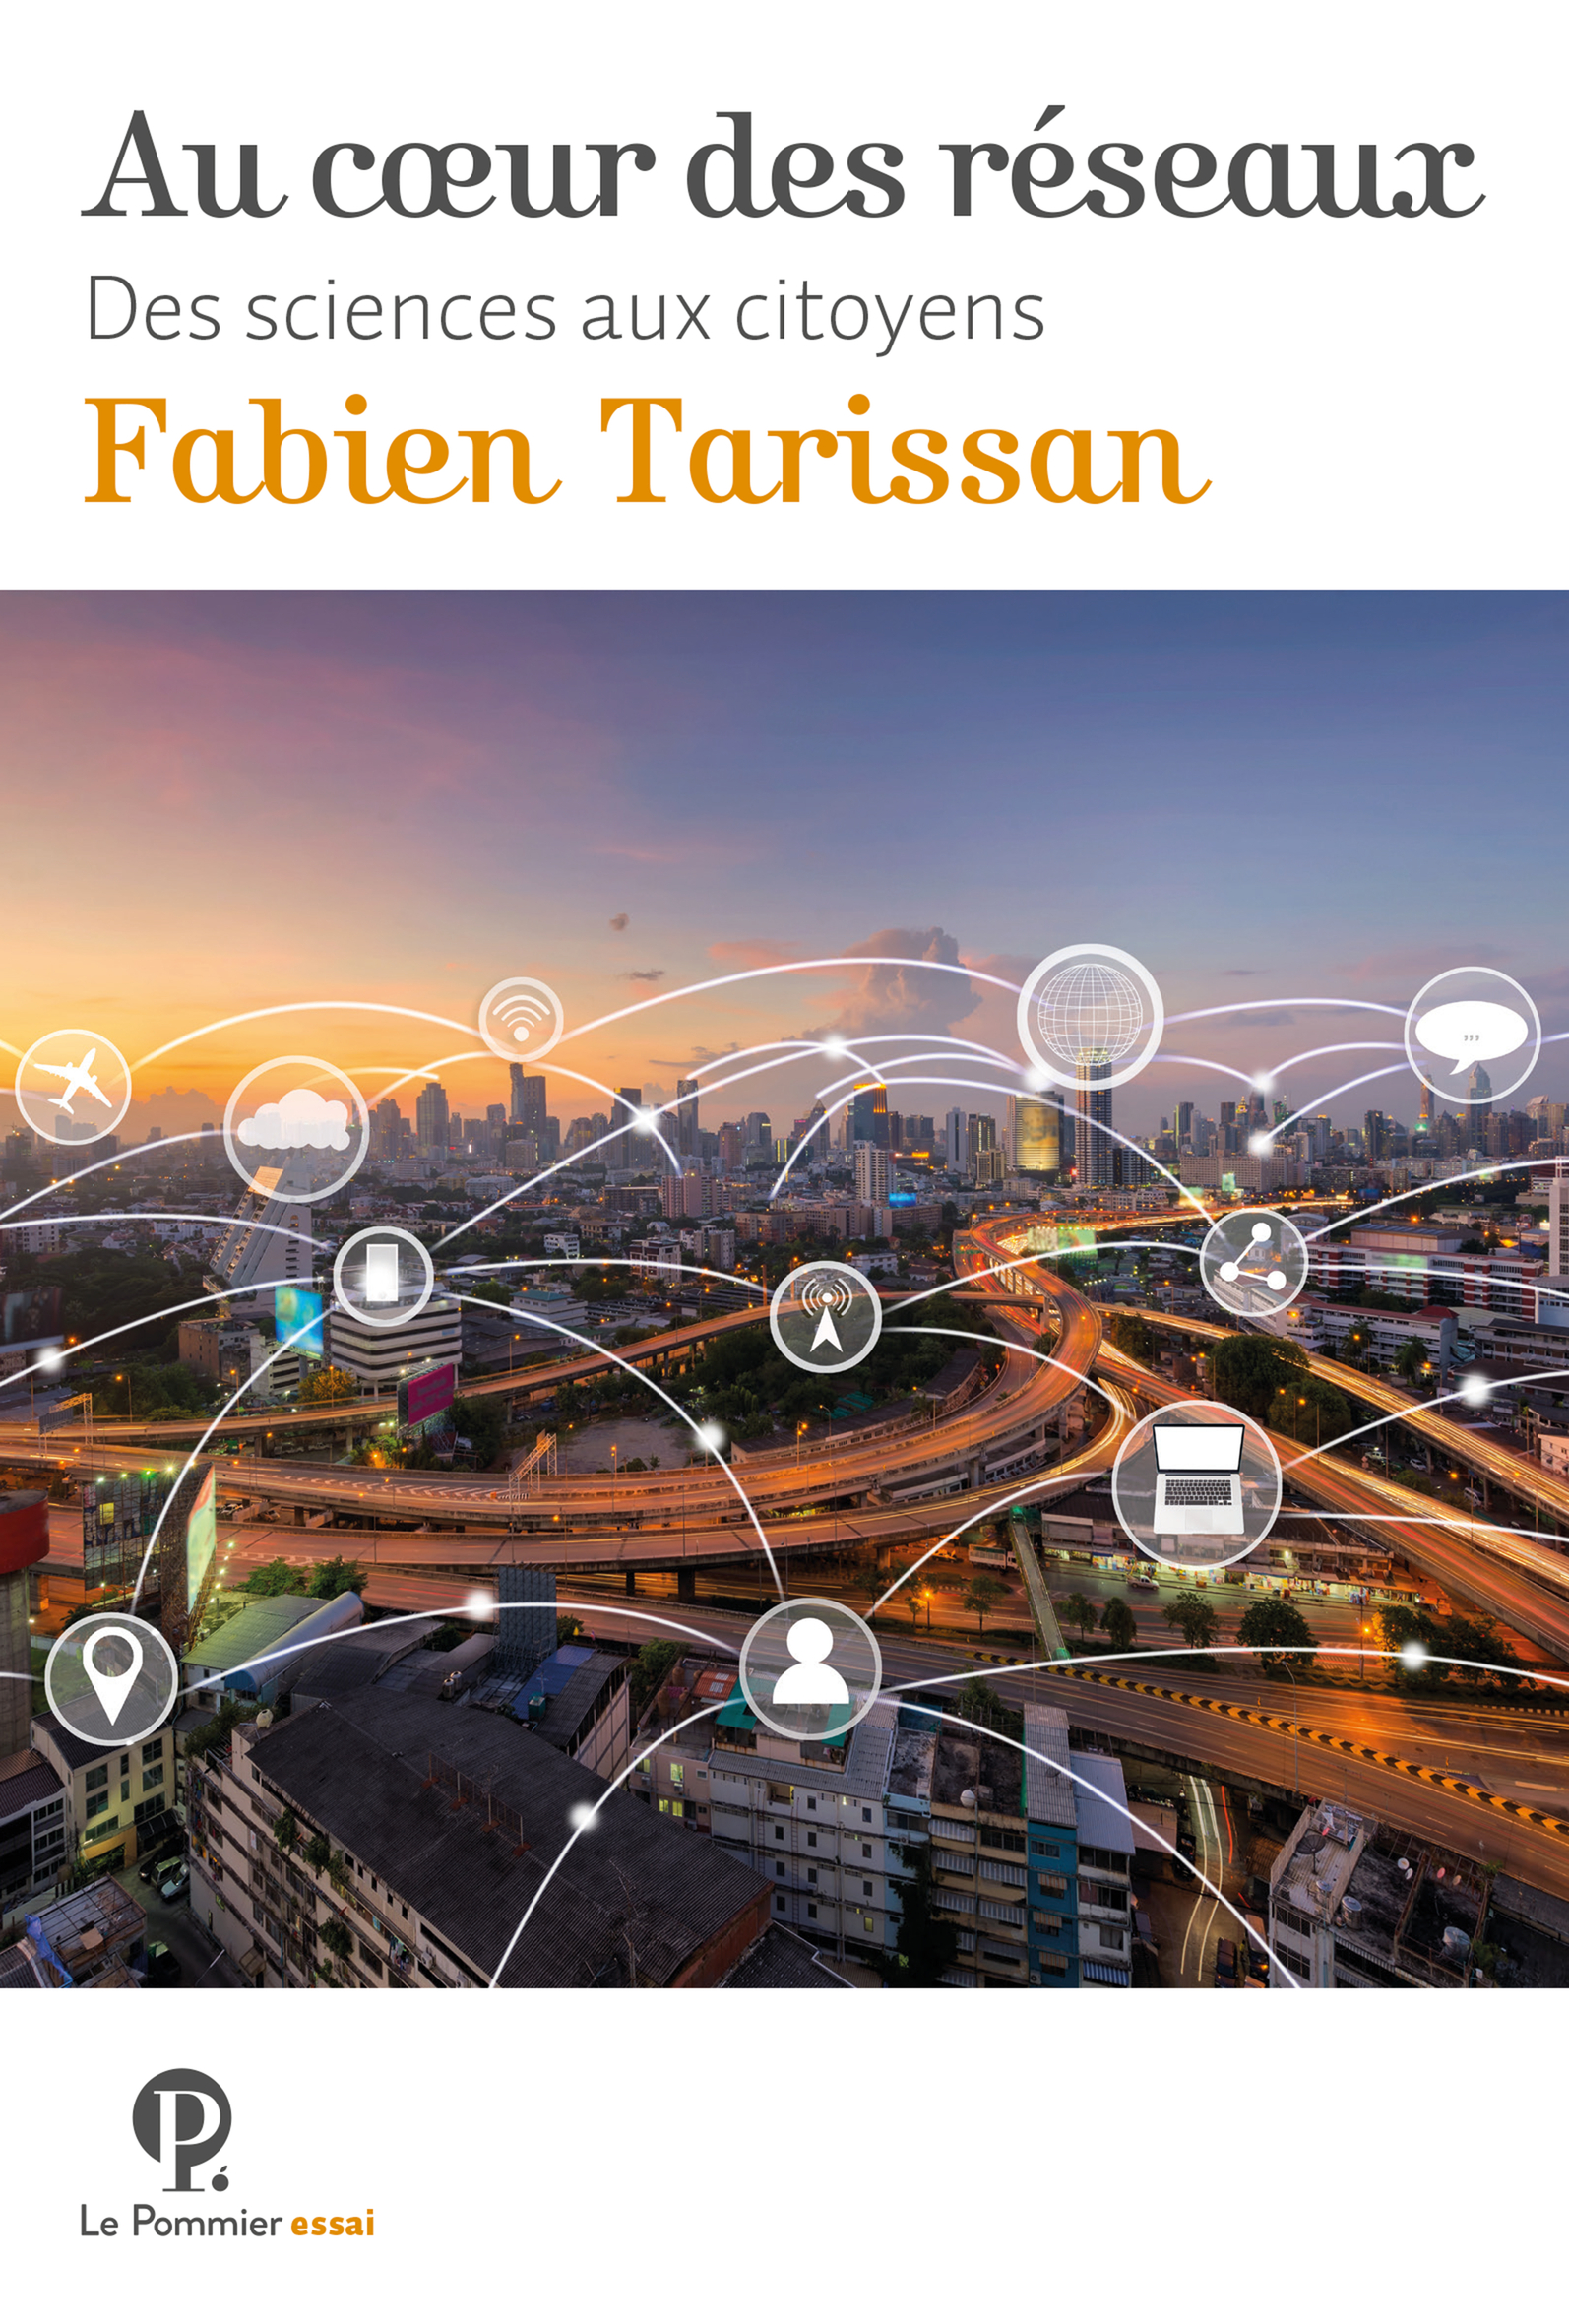
\includegraphics[scale=0.0375]{./Images/Chapter00/tisserand-2019.jpg}\\ \footnotesize\parencite{Tisserand:2019}} 
Fabien \textsc{Tarissan} \linebreak (168 pp, Édition le Pommier, Collection Essai, Mars 2019). Cet ouvrage traite de science, plus particulièrement des réseaux (informatiques mais pas seulement), des algorithmes qui y opèrent et de l'impact qu'ils ont sur notre manière de nous informer en ligne (\textit{fake news}, publicité ciblée, données personnelles, etc.) et de l'économie sous-jacente. Il permet de travailler sur les thématiques réseaux sociaux, objets connectés et internet et réseaux.
\item[L’Hyperpuissance de l’informatique] --- 
\sidegraphic{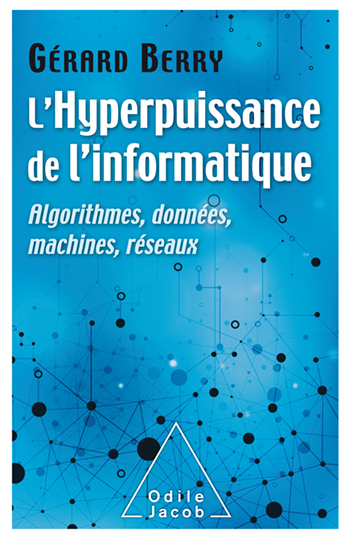
\includegraphics[scale=0.15]{./Images/Chapter00/berry-2017.jpg}\\ \footnotesize\parencite{Berry:2017}} 
Gérard \textsc{Berry} (506 pp, Éditeur Odile Jacob, Collection Sciences, octobre 2017). Ce livre montre de façon non technique comment la science et la technologie informatiques mettent l’information au cœur de l’action, qu’elle soit produite par les humains ou par les machines et conduisent à un nouveau schéma mental différent de celui des siècles précédents, qui confère un pouvoir étonnant à ceux qui le comprennent et l’organisent. Il permet de justifier l'enseignement SNT lui-même et de nourrir le travail sur la pertinence de ces éléments, non sans nourrir les contenus.
\item[Big Data] --- 
\sidegraphic{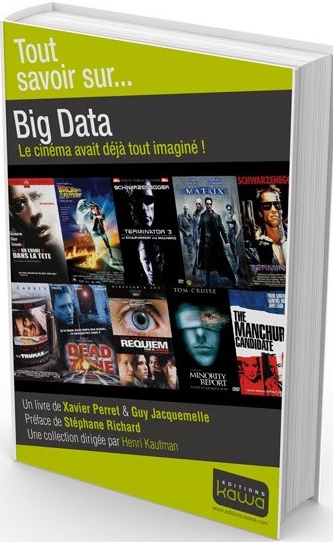
\includegraphics[scale=0.7]{./Images/Chapter00/perret-jacquemelle-2014.png}\\ \footnotesize\parencite{Perret-Jacquemelle:2014}} 
Xavier \textsc{Perret}, Guy \textsc{Jacquemelle} (240 pp, Editions Kawa, Collection : Tout savoir sur, Septembre 2014). Cet ouvrage présente des exemples d’application des \textit{big data}, leurs enjeux et l'importance dans notre société avec une entrée culturelle pluridisciplinaire pour les élèves : des films ; déjà utilisé avec des élèves (en ICN) pour faire réaliser des exposés. Il permet de voir ou revoir des films parfois anciens d’anticipation au travers du prisme de la collecte des données et de leur utilisation. Les auteurs ont créé un cours en ligne ouvert à partir de cet ouvrage.
\end{description}


\vfill\pagebreak\thispagestyle{empty}




























